\documentclass[review]{elsarticle}

\usepackage{lineno,hyperref}
\usepackage{subcaption}
\usepackage{siunitx}
\sisetup{group-separator = {,}}
\usepackage{booktabs}
\usepackage{graphicx}
\usepackage{adjustbox}
\usepackage{appendix}
\usepackage{amsmath} 
\usepackage{scrextend}
\usepackage[hang,flushmargin]{footmisc} 
\usepackage{xcolor}
\usepackage{float}
\usepackage{array,multirow}
\usepackage{hyperref}
\usepackage{setspace}
\usepackage{stmaryrd}
\usepackage{enumitem}
\usepackage{rotating}
\usepackage{adjustbox}
\usepackage{array}
\usepackage{booktabs}
\usepackage{xcolor,colortbl}
\usepackage{amsmath} 
\usepackage{amsfonts} 
\usepackage{amssymb}
\usepackage{makecell}
\usepackage{amsmath}
\usepackage{nicefrac}
\usepackage{todonotes}
\usepackage{multirow}
\modulolinenumbers[1]
\usepackage{lineno}
\usepackage{tikz}
\usepackage{cleveref}
\usepackage{accents} 

\usepackage[final]{changes}
%\usepackage[markup=underlined]{changes}

\usepackage[ruled,vlined,linesnumbered,lined,boxed,commentsnumbered]{algorithm2e}
\newcommand\mycommfont[1]{\footnotesize\ttfamily\textcolor{blue}{#1}}
\SetCommentSty{mycommfont}
\newcommand{\BREAK}{\STATE \algorithmicbreak}
\modulolinenumbers[1]
\setlength{\parindent}{0em}
\journal{Energy Strategy Reviews}
\bibliographystyle{elsarticle-num}
%\bibliographystyle{abbrvnat}

\begin{document}
\begin{frontmatter}

\title{Designing a model for the cost-optimal decommissioning and refurbishment investment decision for gas networks: application on a real test bed in Austria until 2050}
\author[1,2]{Sebastian Zwickl-Bernhard\corref{cor1}}
\ead{zwickl@eeg.tuwien.ac.at}
\author[1]{Antonia Golab}
\author[1]{Theresia Perger}
\author[1,2]{Hans Auer}
\cortext[cor1]{Corresponding author}
\address[1]{Energy Economics Group (EEG), Technische Universität Wien, Gusshausstrasse 25-29/E370-3, 1040 Wien, Austria}
\address[2]{Industrial Economics and Technology Management, Norwegian University of Science and Technology, Gløshaugen, Alfred Getz vei 3, Trondheim, 7491, Norway}

\begin{abstract}
The primary goal of this paper is to investigate the most cost-effective decommissioning and refurbishment investment decision for existing gas networks. An optimization model is developed and tested on a real test bed in an Austrian federal state. The analysis is performed from the network operator's perspective and depicts different network decommissioning or refurbishment options under the decision of supplying or not supplying available gas demands. Whether or not there is ensured supply, we find that smaller gas networks (in terms of pipeline capacity and network length) are needed in the future. Analyzed shadow prices indicate that a balance/trade-off between the cost-optimal gas network design with and without ensured supply could lead to a robust and economically competitive future for downsized gas networks. The results demonstrate that it is necessary to socialize network operators' costs among the remaining consumers connected to the network in the future. This adds a cost component to consumers, which needs to be considered when determining the profitability of sustainable alternatives to natural gas.\\
\end{abstract}

\begin{keyword}
	Gas networks, decommissioning, modeling, cost-optimal, decarbonization
\end{keyword}
\end{frontmatter}

\newpage
\section*{Nomenclature}
\begin{center}
	\renewcommand{\arraystretch}{1.0}
	\centering
	\small
	\begin{tabular}{lm{7.75cm}r}
		Type & Description & Unit\\
		\hline
		Set and index & & \\
		\hline
		{$p \in \mathcal{P}=\{1,\ldots,P\}$} & Pipeline for gas transport, index by $p$\\
		{$n \in \mathcal{N}=\{1,\ldots,N\}$} & Node of the gas network, index by $n$\\
		{$l \in \mathcal{L}=\{1,\ldots,L\}$} & Gas network level (e.g., high-pressure), index by $l$\\
		{$y \in \mathcal{Y}=\{1,\ldots,Y\}$} & Years, index by $y$\\
		{$m \in \mathcal{M}=\{1,\ldots,M\}$} & Months, index by $m$\\
		\hline
		\multicolumn{2}{l}{Primal Decision Variables (Selection)}\\
		\hline
		{$Capex$} & Capital expenditures & \SI{}{EUR}\\
		{$Opex$} & Operational expenditures & \SI{}{EUR}\\
		{$Rev$} & Revenues generated by gas supply & \SI{}{EUR}\\
		{$\gamma_{p,l,y}$} & Capacity of pipeline $p$ at $l$ in $y$& \SI{}{MW}, \SI{}{GW}\\
		{$q^{dem}_{n,l,y,m}$} & Gas demand supplied at $n$ and $l$ in $y$ and $m$ & \SI{}{MWh}, \SI{}{GWh}\\
		{$q_{p,l,y,m}$} & Quantity of gas transported at $p$ and $l$ in $y$ and $m$& \SI{}{MW}, \SI{}{GW}\\
		{$\Pi_{p,l,y}$} & Book value of pipeline $p$ at $l$ in $y$ & \SI{}{EUR}\\
		\hline
		\multicolumn{2}{l}{Dual Decision Variables}\\
		\hline
		{$\lambda^{CO}_{n,l,y,m}$} & Cost-optimal shadow price of gas supply without ensured supply at $n$ and $l$ in $y$ and $m$ & \SI{}{EUR \per MWh}\\
		{$\lambda^{ES}_{n,l,y,m}$} & Cost-optimal shadow price of gas supply with ensured supply at $n$ and $l$ in $y$ and $m$ & \SI{}{EUR \per MWh}\\
		\hline
		\multicolumn{2}{l}{Parameters (Selection)}\\
		\hline
		{$\gamma^{pre}_{p,l,y}$} & Preexisting capacity of pipeline $p$ at $l$ in $y$ & \SI{}{MW}, \SI{}{GW}\\
		{$d^{max}_{n,l,y,m}$} & Maximum gas demand at $n$ and $l$ in $y$ and $m$ & \SI{}{MWh}, \SI{}{GWh}\\
		{$q^{fed}_{n,l,y,m}$} & Quantity of gas fed in at $n$ and $l$ in $y$ and $m$ & \SI{}{MW}, \SI{}{GW}\\
		{$c^{inv}_{l}$} & Specific refurbishment investment costs at $l$  & \SI{}{EUR \per MW \per km}\\
		{$\Pi^{pre}_{p,l,y}$} & Book value of preexisting pipeline $p$ at $n$ in $y$& \SI{}{EUR}\\
		{$y^{inv}_{p,l}$} & Year of refurbishment/decommissioning per $p$ and $l$ & \SI{1}{}\\
		{$\omega$} & Weighted average cost of capital & \SI{}{\%}\\
		{$i$} & Interest rate (for calculating the net present value) & \SI{}{\%}\\
		\hline
	\end{tabular}
\end{center}
\newpage

\section{Introduction}
Adherence to the remaining CO\textsubscript{2} budget of the Paris Agreement requires rapid defossilization of the energy system \cite{rockstrom2017roadmap}. In Europe, the \textit{Fit for 55} package \cite{european_commission_european_2019} and the \textit{EU Green Deal} \cite{greendeal} define the mid- and long-term goals for a transition to a sustainable energy supply until the middle of the century. These goals include a reduction of CO\textsubscript{2} emissions by 55\% compared to those in 1990 by 2030 and climate neutrality in 2050. In light of this, the question of the concrete design of measures to achieve these goals arises \cite{hainsch2022energy}. Numerous scientific works have already been dedicated to the analysis of sustainable alternatives for the provision of energy service needs, which currently rely on fossil fuels. Abas et al. \cite{abas2015review} provide a comprehensive review of fossil fuels as a primary energy source in the energy supply chain and future energy technologies. Corresponding studies, \added[]{(e.g., \cite{hainsch2022energy} and \cite{abas2015review}),} \replaced[]{often}{frequently} focus primarily on the renewable energy technology portfolio that provides energy service needs in the future. We essentially use these as the starting point of our analysis here, investigating implications of expected declining coverage of energy services by natural gas, a fossil fuel, on its transmission and distribution network infrastructure.\vspace{0.35cm}

Natural gas is undeniably one of the pillars of existing energy systems, but it is being fundamentally challenged by the already established and ongoing decarbonization of energy systems. Furthermore, as part of the sustainable transition, natural gas and its role are expected to undergo significant transformation.\footnote{McGlade and Ekins \cite{mcglade2015geographical} state that half of natural gas reserves should remain unused from 2010 to 2050 in order to meet at least the less ambitious 2.0°C climate target from the Paris Agreement.} However, presently, it is not clear which exact trajectory natural gas will take until 2050 \cite{safari2019natural}.\footnote{Exemplarily, Kumar et al. \cite{kumar2011current} see natural gas as an important bridging fuel to a sustainable energy system, in some cases even after 2050. By contrast, Stephenson et al. \cite{stephenson2012greenwashing} propose to abandon the transition fuel characterization of natural gas. D{\'\i}az et al. \cite{diaz2017we} follow this point of view since they find for the electricity sector that natural gas delivers little to no cost savings as a bridging fuel in a system that switches to wind and solar.} Two focal reasons/subjects are (i) various energy sectors currently use natural gas in the provision of energy services (e.g., generation of process heat or as a base material for industrial consumers, centralized generation of electricity and district heating, and decentralized supply of space heating and hot water demands), and it is not clear if and when exactly sustainable alternatives will be economically available, implemented, and realized in sufficient quantities \cite{mohseni2013competitiveness, gorre2019production}. (ii) Synthetic gases (including hydrogen) are seen as a promising alternative or supplement to natural gas usage, as they could be fed into existing transmission and distribution gas network infrastructure, although there are valid uncertainties regarding its amount of technical as well as economic potentials \cite{lux2020supply, blanco2018potential}. Because of that, the question is not only which energy sectors and energy services remain to use the limited quantities of natural (following the trend of defossilization) and synthetic (because of limited potentials gas) but also what gas network infrastructure will continue to be needed for their transport and distribution.\vspace{0.35cm}

The goal of this paper is to contribute to scientific research on its future development and trajectory of gas network infrastructure with the expectation of decreasing natural gas demands and increasing the integration of green gases, such as synthetic gas and hydrogen. The emphasis is on gas network infrastructure, which ensures that various energy service needs (e.g., residential building heat, and industrial process heat) are met. This raises the question of which gas network infrastructure is required to meet non-substitutable natural gas demands when considering possible stand-alone natural gas supply options (e.g., delivery of liquefied natural gas by truck) \added{in order to avoid significant economic loss and stranded assets in the future. To meet demand, the network can transport either imported gas volumes or locally produced green gases such as biomethane.} Nonetheless, even if stand-alone solutions are viable alternatives in some cases, arbitrariness regarding the trajectory decisions of gas networks must be avoided, as they are not only assigned to critical infrastructure but also regulated and subject to long-term energy planning (lock-in effect).\vspace{0.35cm} 

The primary objective of this work is to investigate the cost-effective trajectory of gas network infrastructure from a systemic viewpoint under a long-term planning horizon. Given necessary refurbishment investments in existing gas network infrastructure and pipelines due to their technical lifetimes, the main research question is which decommissioning and refurbishment investment decisions result in a cost-effective gas network infrastructure by 2050. Equally important in the analysis is the network operator's trade-off decision regarding whether available gas demands within the network area are supplied or not, as decommissioning of existing gas pipelines can be cost-effective but results in unsupplied gas demands. Consequently, three different model runs are performed, allowing a thorough comparison of various handling options in terms of gas demands not met by the network infrastructure.\footnote{Grid operator usually is a regulated entity. Thus, finally, it is a regulatory question/decision which cannot be taken by the grid operator alone (regulator).} Accordingly, analysis relies heavily on the shadow prices of gas supply at the local level within the network's nodes. \added{At present, existing studies on gas network infrastructure are insufficient, and the corresponding literature has not yet conducted a comprehensive comparison of different sub-policy implications for handling future gas demands by a quantitative analysis.}\vspace{0.35cm}

The method used is the development of a linear optimization model. Thereby, the objective function is to minimize the network operator's net present value over time. Particularly, the optimal solution of the model includes the decommissioning and refurbishment investment decision of parts of the network and single pipelines. This includes deciding whether or not to supply available gas demand. The dual variables of the local gas balance constraints allow us to assess the techno-economic range of supply alternatives for each node in the network.\vspace{0.35cm}

The numerical example examined is a small portion of the existing Austrian gas network infrastructure in the NUTS2 region Vorarlberg, Austria. This area is distinguished by a wide range of energy service requirements that are met by natural gas (e.g., residential, and industry). Furthermore, the gas network infrastructure includes not only high- and mid-pressure network connections but also cross-border connections to neighboring countries Germany and Lichtenstein (i.e., transmission network level). There is also the possibility of producing green gas and injecting it into the existing gas network infrastructure.\vspace{0.35cm}

The paper is organized as follows. Section \ref{stateoftheart} provides an overview of the current state-of-the-art in scientific literature and outlines the novelties of this work beyond existing research. Section \ref{methodology} presents the materials and methods developed in this work, including, the model's mathematical formulation and description of different model runs. Section \ref{results} presents the results of this work encompassing different handlings of gas demands within the network. Section \ref{conclusions} synthesizes and discusses the results, concludes the work, and gives an outlook for future research.  
\section{State-of-the-art and progress beyond}\label{stateoftheart}
This section provides an overview of relevant scientific literature for this paper's scope. It emphasizes two essential subjects, namely, the role of natural and green gases in sustainable energy systems (Section \ref{state:1}) and the modeling of gas networks from a system perspective point of view (Section \ref{state:2}). The novelties of this work and progress beyond state-of-the-art are also presented (Section \ref{state:3}). 

\subsection{Natural and green gases in sustainable energy systems}\label{state:1}
It is debatable whether natural gas will play a significant role in the energy transition over the next few decades, and if so, under what conditions. Gürsan and Gooyert \cite{gursan2021systemic} provide a recent and concise review of the state-of-the-art in the role of natural gas in reducing CO\textsubscript{2} emissions from energy systems. Kotek et al. \cite{kotek2019european} conduct a study on the European natural gas infrastructure in the context of energy transition. Already in 2012, Stephenson et al. \cite{stephenson2012greenwashing} discuss natural gas as a transition fuel in the sustainable transformation of energy systems. They concluded that a natural gas climate solution is unsubstantiated. This is also reflected in a large number of studies on cost-optimal energy supply until 2050. Auer et al. \cite{auer2020development}, for example, investigate the European energy supply until 2050 for various decarbonization scenarios under the remaining European fraction of the CO\textsubscript{2} budget and discover that natural gas is almost completely replaced in the primary energy demand in 2040.\vspace{0.35cm}

Green gases are becoming increasingly important, as evidenced by not only the results of Auer et al. for Europe but also, those of Zhang et al. \cite{zhang2022potential} for China. Against this background, it is certainly possible to see existing natural gas networks as a crucial part of the energy transition to transport and deliver green gases. Recently, Quintino et al. \cite{quintino2021aspects} elaborate on aspects of green gas introduction in natural gas networks. Dodds and McDowall \cite{dodds2013future} examine the long-term future of gas networks and state that the most cost-effective strategy might be to convert the networks to deliver green gases. Interestingly, Dodds and McDowall find in their scenarios that hydrogen injection into gas networks has only a small role and low impact on gas networks. \added[]{Kolb et al. \cite{kolb2021scenarios} examine the integration of green gases into a natural gas market. They provide not only a comprehensive literature review of the future role of renewable gases but also show that the carbon price is one of the most promising ways to promote renewable gases.} \deleted{Similarly,} Mac Kinnon et al. \cite{mac2018role} investigate the role of natural gas networks in mitigating greenhouse gas emissions. Gillessen et al. \cite{gillessen2019natural} elaborate on the role of natural gas as a bridge to sustainable energy systems and related infrastructure expansion of gas networks. Gondal \cite{gondal2019hydrogen} studies the hydrogen integration into gas transmission networks.\footnote{Particularly, Gondal states that (i) at the transmission network level, compressors are the determinant element and limit the value of hydrogen by 10\%; (ii) at the distribution network level, pipelines and storage elements allow shares up to 50\% of hydrogen; and (iii) at the level of end use appliances, a tolerant range and share of 20-50\% of hydrogen is possible.}\vspace{0.35cm}

Nonetheless, although the expected potential of green gases exists, it is nowhere large enough to replace the current amount of natural gas in the energy supply. Accordingly, the discussion of existing natural gas networks may and should include decommissioning as part of the solution space. Furthermore, this possibility should no longer be seen as a taboo subject but rather as a real decision option that can even be argued from a techno-economic point of view. Giehl et al. \cite{giehl2021modelling} examine cost-optimal gas networks and focus particularly on the distribution network level, finding a declining need for gas distribution networks in their future scenarios. Zwickl-Bernhard and Auer \cite{zwickl2022demystifying} present the decommissioning of a gas distribution network in an urban area at the community level. Feijoo et al. \cite{feijoo2018future} find risks of underutilization of gas networks (i.e., pipeline capacities) in a low-carbon future economy even at the interstate and transmission level. Brosig et al. \cite{brosig2017benchmark} compares the cost-effectiveness of different future pathways between expansion and decommissioning of the gas grid network.\vspace{0.3cm}

In this context, local renewable energy sources and technologies are becoming increasingly important. For example, district heating contributes in densely populated and urban areas to the decrease of natural gas in the supply of energy service needs. Möller and Lund \cite{moller2010conversion} examine the conversion of individual natural gas heating units to district heating. Hofmann et al. \cite{hofmann2014potential} show the use of geothermal sources for heat generation for both residential and industrial. At the national level, Geyer et al. \cite{geyer2021100} presents scenarios, energy carriers and infrastructure requirements for a completely renewable energy-based industry sector. Rahnama et al. \cite{rahnama2021pulp} show particularly the reduction of gas demands and associated CO\textsubscript{2} emission for the pulp and paper industry by electrification of energy service needs. Bachner \cite{bachner2020risk} et al. focus on the replacement of gas and other fossil fuels in the steel and electricity sector from a macroeconomic perspective\footnote{In the context of a decarbonized electricity supply, Qadrdan et al. \cite{qadrdan2015impact} investigate the impact of transitioning to a low-carbon electricity sector on gas network infrastructure. Particularly, the authors focus on the gas network in Great Britain and find that despite the declining gas demand, the peak gas demand remains unchanged.}.\vspace{0.35cm}

Findings of the literature in the previous paragraph indicate that large portions of natural gas demands can, in principle, be substituted by sustainable alternatives. Against this background and considering that natural gas networks are regulated entities of the energy system, are capital intensive, and therefore require long-term strategies or planning, avoidance of stop-and-go policy is crucial. Exemplarily, Then et al. \cite{then2020impact} study the operator strategy and economic viability of gas networks in face of decreasing gas demands. Hickey et al. \cite{hickey2019there} identify significant challenges and risks to policymakers and investors in using gas networks in sustainable energy systems encompassing the risk of stranded assets resulting not only from declining gas demand but also from changes in regulation and how tariffs are allocated. Hausfather \cite{hausfather2015bounding} focuses on the policy decisions for natural gas and its network infrastructure until 2030 as they irreversibly impact the future of natural and synthetic gas in the period 2030 to 2050\footnote{Moreover, Hausfather concludes that policy decisions are needed leading to decarbonization of natural gas no later than 2030.}. Glachant et al. \cite{glachant2014gas} study and identify the fundamental reasons for diverging gas network and market developments. Mos{\'a}cula et al. \cite{mosacula2018designing} propose a novel methodology for gas network charges design, which builds on economic efficiency as the main principle.\vspace{0.3cm}

\added[]{A few selected works on energy and network security of natural gas are mentioned here without claiming completeness. Hutagalung et al. \cite{hutagalung2017economic} deal with investments in natural gas infrastructure and their implications on energy security and economic growth.} Tata and DeCotis \cite{tata2019natural} focus on risks and responsibilities associated with natural gas infrastructure development. \added[]{They do not advocate for or against using natural gas but argue that all energy supply options have risks that must be considered when deciding which fuel to use.} Sacco et al. \cite{sacco2019portfolio} analyze the risks associated with maintenance gas networks. Sesini et al. \cite{sesini2020impact} assess resilience and security in gas network systems. \replaced[]{They examine the impact of a real demand shock on the European natural gas network, focusing on liquefied natural gas and storage.}{The key findings can be summarized as decisions on natural gas infrastructure development should not be made through a single-lens view.}

\subsection{Modeling gas networks}\label{state:2}
Particularly, the previous paragraph regarding the challenges and risks of long-term planning of gas networks provides the starting point for this section dedicated to modeling and simulation of gas networks. R{\'\i}os-Mercado \cite{rios2015optimization} present a comprehensive state-of-the-art review on the optimization of natural gas networks encompassing both the transmission and distribution network level. Osiadacz and Gorecki \cite{osiadacz1995optimization} provide an even broader summary of gas network optimization modeling approaches. Particularly, they mention heuristic, continuous and discrete methods of the optimal design of gas networks. Feijoo et al. \cite{feijoo2016north} propose a long-term partial equilibrium model that allows for endogenous
gas network infrastructure expansion and nonlinear cost functions. Fügenschuh et al. \cite{fugenschuh2011gas} develop an optimization model with quadratic formulation. Fodstad et al. \cite{fodstad2016stochastic} and Aßmann et al. \cite{assmann2019decomposable} use stochastic optimization including gas demand uncertainties in the optimization of gas networks. Latter use a decomposable robust two-stage optimization model. Von Wald et al. \cite{von2022optimal} propose a multiperiod planning framework for decarbonization of integrated gas and electric energy systems. \added[]{Similarly, the work of Cavana et al. \cite{cavana2021electrical} is aimed at sector coupling. In their work, the authors emphasize the ability of the gas network for hydrogen blending to enable greater integration of renewable energy.}\vspace{0.35cm}

The long-term planning of gas networks is exemplarily shown by Hubner and Haubrich \cite{hubner2008long} and Giehl et al. \cite{giehl2021modelling}. \deleted[]{The latter proposes a greenfield approach and optimization model for gas networks without considering the existing network infrastructure (i.e., from scratch).} Mikolajkov{\'a} et al. \cite{mikolajkova2017optimization} show the optimization of a natural gas distribution network with the potential future extension of the transmission network level. Kashani et al. \cite{kashani2014techno} present the techno-economical and environmental optimization of natural gas network operation. Farsi et al. \cite{farsi2007cost} show a national case study regarding the cost efficiency of gas distribution networks. Particularly, they emphasize the impact of customer density and network size in the Swiss gas distribution sector. Odetayo et al. \cite{odetayo2018real} show the modeling flexibilities of gas networks for energy system operation. Di{\'e}guez et al. \cite{dieguez2021modelling} show the modeling of decarbonization transition in a national integrated energy system including hourly operational resolution of gas networks. Yusta and Beyza \cite{yusta2021optimal} emphasize the modeling of large-scale gas storage facilities by a dynamic approach. Kerdan et al. \cite{kerdan2019modelling} link a spatially resolved gas infrastructure optimization model with an energy system model.\vspace{0.3cm}

\added[]{This paragraph concludes the literature review with a discussion of existing approaches and models used to achieve similar objectives to this study. It becomes clear that there are relevant studies in this area but also that there is currently a lack of work in the literature explicitly addressing decommissioning and reinvestment decisions for gas networks. For example, Giehl et al. \cite{giehl2021modelling} provide an in-depth analysis of the impact of energy system decarbonization on gas distribution networks. For a German case study, they show a decreasing need for gas distribution networks until 2050. A strength of their approach is certainly the comprehensive model they use, called "DINO". However, they use a greenfield approach and do not consider existing networks and pipelines. Then et al. \cite{then2020impact} examine the impact of different gas network operator strategies on gas network profitability in the face of declining demand. They carry out comprehensive gas network planning under different strategies but focus on network charges in terms of strategy. They also use commercial software and estimate a functional relationship between required network length and demand. Bouacida et al. \cite{bouacida2022impacts} investigate the impact of decarbonization on gas networks and costs. Based on a review of French and German decarbonization scenarios, they examine the impact on gas networks and estimate the change in gas prices for end users. They also argue that the latter will increase, accelerating the substitution of natural gas. In their paper, Oberle et al. \cite{oberle2022can} ask whether industrial gas demand can keep gas distribution networks alive or not? They focus on the development of gas demand in Germany until 2050. However, their analysis focuses more on the implications for gas networks than detailed network modeling. Given this, there is no existing work proposing a method that could, to the best of our knowledge, be used to address the objectives of this work.}

\subsection{Progress beyond the state-of-the-art}\label{state:3}
Based on the literature review, the novelties of this work can be summed up as follows:
\begin{itemize}
	\item A cost-effective trajectory of existing gas network infrastructure is modeled considering the expectation of both declining gas demands resulting from the defossilization of energy services and the increasing but limited integration of green gases, such as synthetic gas and hydrogen.  
	\item Since existing gas network infrastructure requires the refurbishment of its gas pipelines due to the expiration of the technical lifetime, it is shown how the gas network operator decides from a techno-economic point of view between decommissioning and refurbishment investment of gas pipelines at different network and pressure levels. Especially, the transmission, high-pressure, and mid-pressure network levels are analyzed. \added[]{The assumed pressure levels are between} \SI{64}{bar} \added[]{for the transmission and high-pressure network levels, and} \SI{4}{bar} \added[]{for the mid-pressure network level.}
	\item The optimization of a cost-effective trajectory of existing gas network infrastructure includes, the gas network operator's decision between supplying or not supplying available gas demand (i.e., disconnection from the gas network by decommissioning gas pipelines and implicitly implementing stand-alone gas supply alternatives). Particularly, the long-term planning horizon of the model allows for investigating this trade-off decision between investment/capital costs, related book values, and expected revenue and purchase streams for individual gas pipelines.
	\item The application of the proposed model on a real test bed in a NUTS2 region in Austria until 2050 provides useful insights that can be used directly by decision and policymakers. The investigated test bed is representative of other gas networks since it comprises, on the one hand, gas demands that are supplied in different end-user sectors, and, on the other hand, encompasses different gas network/pressure levels. Accordingly, the transmission network level is also considered as the test bed gas network is linked to neighboring countries.  
\end{itemize}
 \section{Materials and methods}\label{methodology}
 This section explains the proposed methodology. First, Section \ref{Met:Intro} introduces the model. Then, Section \ref{Met:Equations} presents the mathematical formulation in detail. Section \ref{runs} explains the different model runs and defined scenarios. Section \ref{testbed} provides the test bed description and shows the gas networks in Vorarlberg, Austria, in detail, and Section \ref{label:inputs} presents the input data. Section \ref{label:limitation} discusses the limitations of the model. Finally, Section \ref{environment} deals with the open-source programming environment and the computation time of the model. 
 
 \subsection{Introduction of the model}\label{Met:Intro}
 Figure \ref{fig:methodology} provides an overview of the method, including the interrelationships between the inputs (left), the \replaced{model}{modeling framework} (middle), and the outputs (right). Generally, the inputs (and thus parameters) can be divided into three different categories, namely, technical parameters (e.g., existing pipeline capacity per network/pressure level and the year of construction), economic parameters (e.g., refurbishment investment costs per pipeline), and further empirical data needs (e.g., gas demand and supply at the local community level and seasonal gas storage capacities). The \replaced[]{model}{modeling framework (CANCEL)} is developed as a linear program and is based on graph theory. It emphasizes the high spatial resolution in modeling. Particularly, a single node in the gas network graph corresponds to a community and covers an area of approximately \SI{40}{km^2} on average. The temporal resolution and thus investment planning horizon are until 2050, whereas an individual year is monthly resolved. \replaced[]{The model outputs include the optimal investment and dispatch decisions.}{Since the modeling framework is an investment and dispatch model, the outputs can also be divided into these catergories.} The outputs related to the investment decision are particularly the decommissioning and refurbishment investment decision per pipeline and gas network level. Additionally, the outputs encompass the dispatch of the gas networks on a monthly resolution. This includes the utilization of pipelines and particularly the gas demand and gas demand not supplied per community. 
 
  \begin{figure}[h]
 	\centering
 	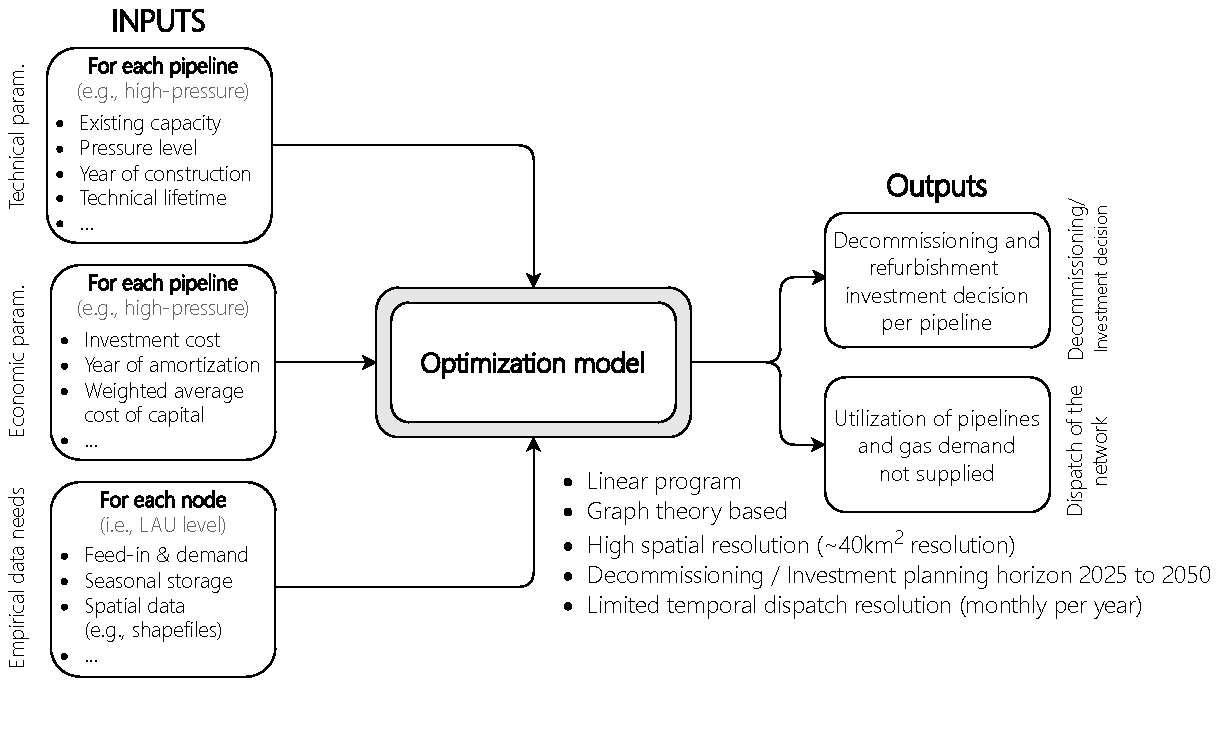
\includegraphics[width=1\linewidth]{figures/flowchart.pdf}
 	\caption{Overview of the method}
 	\label{fig:methodology}
 \end{figure}
 
 \subsection{Mathematical formulation}\label{Met:Equations}
 This section is dedicated to providing a detailed mathematical formulation of the \replaced[]{model}{modeling framework}. We start with the objective function and have deliberately chosen the further order of equations so that the following equation builds on the previous one as far as possible. \added[]{In addition to the detailed description of the equations below, Table} \ref{tab:brief} in \ref{app_overview} \added[]{summarizes the main equations of the model with a qualitative explanation.}\vspace{0.35cm}
 
 Equation \ref{objective} shows the objective function of the model where $Capex$ is the net present value of the capital expenditures, $Opex$ of the operational expenditures, $Rev$ of the revenues from the supply of gas demands, and $Purch$ of purchasing gas. $Capex$ and $Opex$ represent the decommissioning and investment decision, whereas $Rev$ and $Purch$ the dispatch of the gas networks.  
 \begin{align}\label{objective}
  	\underset{x}{\mathrm{min~}} Capex + Opex - Rev + Purch
  \end{align}
Additionally, $x$ represents the decision variables of the model. \added{All costs and prices are nominal.} Equation \ref{discount} shows the calculation of the discount factor per year $y$ ($\alpha_y$), where $i$ is the interest rate and $y_0$ is the reference year. 
\begin{align}\label{discount}
	\alpha_y = \frac{1}{(1+i)^{y-y_0}}
 \end{align}
Building upon, $Capex$ is calculated as shown in Equation \ref{eq:capex} where $\omega$ is the weighted average cost of capital and $\Pi_y$ is the book value of the pipelines in $y$.
\begin{align}\label{eq:capex}
	Capex = \sum_{y}^{y_{end}-1} \alpha_y \cdot \omega \cdot \Pi_y + \underbrace{\alpha_{y_{end}} \cdot \Pi_{y_{end}}}_{\text{early depreciation}}	
\end{align}
Similarly, $Opex$ is calculated as shown in Equation \ref{eq:opex} where $\lambda_y$ is the fixed (operating) costs of the pipelines in $y$. 
\begin{align}\label{eq:opex}
	Opex = \sum_{y} \alpha_y \cdot \lambda_y
\end{align}
Equation \ref{eq:lambda} shows the calculation of the $\lambda_y$ where $c^{fix}_{l}$ is the specific fixed (operating) costs per $l$ and $\gamma_{l, y}$ is the installed pipeline capacity per $l$ in $y$.
\begin{align}\label{eq:lambda}
	\lambda_y = \sum_{l} c^{fix}_{l} \cdot \gamma_{l, y}
\end{align}
Equation \ref{eq:gamma} shows the calculation of $\gamma_{l, y}$ where $\gamma_{p,l,y}$ is the installed pipeline capacity at $p$ and $l$ in $y$ and $P_{l}$ the subset of all pipelines at $l$. \added[]{$\Lambda_{p}$ is a scaling factor. It is needed because the parameter $c^{fix}_{l}$ is defined for a representative pipeline length for each pressure level. These representative pipeline lengths are 50km and 25km for the high-pressure and mid-pressure network levels respectively. For example, if a pipeline $p$ at the high-pressure network level has a length of 50km, then the scaling factor $\Lambda_{p}$ is equal to 1. Note that $\Lambda_{p}$ is known a priori (because the length of pipelines are known) and is a parameter of the model.}
\begin{align}\label{eq:gamma}
	\gamma_{l, y} = \sum_{p \in P_{l}} \Lambda_{p} \cdot \gamma_{l, y, p}
\end{align}
Equation \ref{eq:total_capacity} defines the capacity of a pipeline $p$ at $l$ in $y$ where $\gamma^{pre}_{p,l,y}$ is the preexisting capacity and $\gamma^{ref}_{p,l,y}$ is the refurbished capacity of $p$ at $l$ in $y$. 
\begin{align}\label{eq:total_capacity}
	\gamma_{p,l, y} = \gamma^{pre}_{p,l,y} + \gamma^{ref}_{p,l,y}
\end{align}
Similarly, Equation \ref{eq:total_book_value} defines the book value of a pipeline $p$ at $l$ in $y$, where $\Pi^{pre}_{p,l,y}$ is the book value of the preexisting pipeline (capacity), $\Pi^{ref}_{p,l,y}$ of the refurbished capacity of $p$ at $l$ in $y$, and $f^{ref}_{p,l}$ the discount factor at $p$ and $l$.
\begin{align}\label{eq:total_book_value}
	\Pi_{p,l,y} = \Pi^{pre}_{p,l,y} + f^{ref}_{p,l} \cdot \Pi^{ref}_{p,l,y^{inv}_{p,l}}
\end{align}
Equation \ref{eq:tbv} sums the book values of all pipelines and network levels to obtain the total book value per $y$ ($\Pi_y$).
\begin{align}\label{eq:tbv}
	\Pi_{y} = \sum_{p} \sum_{l} \Pi_{p,l,y}
\end{align}
The following equation defines the refurbished installed capacity per $p$ at $l$ in $y$ resulting from the refurbishment (or decommissioning) decision in the year of the decision ($y^{inv}_{p,l}$).
\begin{align}\label{9}
	\gamma^{ref}_{p,l,y} = \begin{cases}
		0 & \quad:\forall y~|~y<y^{inv}_{p,l}\\
		\gamma^{ref}_{p,l,y-1} & \quad:\forall y~|~y>y^{inv}_{p,l}
	\end{cases}
\end{align}
Equation \ref{eq:bvalue_ref} calculates the book value of the refurbishment investment at $p$ and $l$ in $y^{inv}_{p,l}$.
\begin{align}\label{eq:bvalue_ref}
	\Pi^{ref}_{p,l,y^{inv}_{p,l}} = c^{inv}_{l} \cdot \gamma^{ref}_{p,l,y^{inv}_{p,l}}
\end{align}
Equations \ref{exp} and \ref{imp} define the total gas export and import from $n$ at $l$ in $y$ and $m$ where $q_{p,l,y,m}$ is the amount of gas transported by $p$ at $l$ in $y$ and $m$. Additionally, $P^{exp}_{n,l}$ and $P^{imp}_{n,l}$ define the subsets containing all pipelines that can export and import gas from $n$ at $l$.
\begin{align}
	q^{exp}_{n,l,y,m} = \sum_{p \in P^{exp}_{n,l}} q_{p,l,y,m} \label{exp}\\
	q^{imp}_{n,l,y,m} = \sum_{p \in P^{imp}_{n,l}} q_{p,l,y,m} \label{imp}
\end{align}
Equations \ref{bound1} and \ref{bound2} set the lower and upper bound of the amount of gas transported with respect to the installed pipeline capacity.
\begin{align}
	q_{p,l,y,m} \leq \gamma_{l, y, p} \label{bound1}\\
	-q_{p,l,y,m} \leq \gamma_{l, y, p} \label{bound2}
\end{align}
The last two equations underline that a pipeline in the model has a certain direction in which the amount of gas transported is counted positively. Therefore, this direction defines for a node $n$ whether a pipeline $p$ is considered positively in the import or export balance (compare Equations \ref{exp} and \ref{imp}). Exemplarily, a pipeline $p$ could be considered in the export sum of a node $n$ on the one hand with a positive value if $p$ in fact exports gas from $n$ but on the other hand with a negative value if $p$ imports gas to $n$ in the dispatch of the model decision\footnote{We use this approach to prevent binary decision variables. Particularly, binary decision variables increase the computation time of graph-theory based models significantly. For more information, we refer to Kotzur et al. \cite{kotzur2021modeler} and their comprehensive review on how to handle complexity in energy system optimization.}.\vspace{0.35cm}

Equation \ref{eq:balance} shows the general formulation of the balance constraint at $n$ where $q^{sto}_{n,l,y,m}$ is the amount of gas from or to storage. Particularly, this equation is defined for each network level $l$. The coupling of different network levels (e.g., the high- and mid-pressure network levels) is considered implicitly in the definition of the different gas demand variables (see Equation \ref{eq:demand} below). Additionally,  $\xi_m$ is a scaling (or transformation) factor that is defined for each month and is used to couple total values per month (e.g., $q^{dem}_{n,l,y,m}$) and peak values.\footnote{It reflects the fact that Equation \ref{eq:balance} encompasses variables that are associated with nodes ($q^{fed}_{n,l,y,m}$, $q^{dem}_{n,l,y,m}$, $q^{sto}_{n,l,y,m}$) modeled at a monthly resolution and with lines ($q^{exp}_{n,l,y,m}$, $q^{imp}_{n,l,y,m}$) modeled at a hourly resolution.}
\begin{align}\label{eq:balance}
	q^{fed}_{n,l,y,m} - q^{dem}_{n,l,y,m} - \xi_m \cdot \left(q^{exp}_{n,l,y,m} + q^{imp}_{n,l,y,m}\right) + q^{sto}_{n,l,y,m}= 0
\end{align}
Exemplarily, Equation \ref{eq:demand} shows the calculation of the gas demand at network level $l$, where $q^{del}_{n,l',y,m}$ is the amount of gas delivered from network level $l$ to $l'$ and $q^{dem,loc}_{n,l,y,m}$ is the local gas demand supplied at $n$. For example, $l$ could correspond to the transmission network level and $l'$ to the high-pressure network level. Note that the pressure in pipelines at $l$ is higher than at $l'$.
\begin{align}\label{eq:demand}
	q^{dem}_{n,l,y,m} = q^{dem,loc}_{n,l,y,m} + q^{del}_{n,l',y,m}
\end{align}
Equation \ref{eq:notsupplied} is the essential demand constraint and sets the upper bound of the decision variable $q^{dem,loc}_{n,l,y,m}$ to the maximum available gas demand $(d^{max}_{n,l,y,m})$, in which is defined as an input parameter. 
\begin{align}\label{eq:notsupplied}
	q^{dem,loc}_{n,l,y,m} \leq d^{max}_{n,l,y,m}
\end{align}
Particularly, Equation \ref{eq:notsupplied} allows the model by its mathematical operator with the less than or equal sign $(\leq)$ to decide between supplied and not supplied gas demand at the nodal level. This decision is in the foreground of the conducted analysis here, which is why we use particularly Equation \ref{eq:notsupplied} to define different model runs and thus scenarios. Accordingly, the model runs and scenarios differ by the individual specification of the demand constraint (i.e., $\leq$ or $=$ and $d^{max}_{n,l,y,m}$ as the upper bound of the equation). We refer to a detailed description of the model runs and scenarios in Section \ref{runs}.\vspace{0.3cm}

The (total) quantity of gas fed at $l'$ is defined as stated in Equation \ref{eq:source} where $q^{fed,local}_{n,l',y,m}$ is the quantity of gas fed directly from $n$. 
 \begin{align}\label{eq:source}
 	q^{fed}_{n,l',y,m} = q^{fed,local}_{n,l',y,m} + q^{del}_{n,l',y,m}
 \end{align}
Equation \ref{eq:storage} defines the balance constraint of a storage unit. Contrary to most storage constraints, we do not consider different efficiency values for the charge and discharge. Hence, a single variable can be used. Additionally, $q^{sto,soc}_{n,l,y,m}$ is the state of charge. $\eta$ is the storage efficiency and thus models the losses with respect to the storage of gas between 2 months. 
\begin{align}\label{eq:storage}
		q^{sto,soc}_{n,l,y,m} = \eta \cdot q^{sto,soc}_{n,l,y,m-1} + q^{sto}_{n,l,y,m}
\end{align}
Equation \ref{eq:revenues} calculates the revenues created by the local gas demand supplied where $p^{loc}_{l,y}$ is the price. \added[]{The latter includes the gas price and the network charge.}
\begin{align}\label{eq:revenues}
	rev_{n,l,y,m} = p^{loc}_{l,y} \cdot q^{dem,loc}_{n,l,y,m}
\end{align}
Accordingly, the revenues ($Rev$ from the objective function in Equation \ref{objective}) are calculated as shown in Equation \ref{eq:total_revenues}.
\begin{align}\label{eq:total_revenues}
	Rev = \sum_{y} \sum_{n} \sum_{l} \sum_{m} \alpha_y \cdot rev_{n,l,y,m}
\end{align}
$Purch$ is calculated as shown in Equation \ref{eq:purchase}, where $p^{gas}_{y,m}$ is the gas price in $y$ and $m$. \added[]{As a result, the gas network operator only receives revenue through the network tariff. This becomes evident when comparing Equations \ref{eq:revenues} and \ref{eq:purchase}.}
\begin{align}\label{eq:purchase}
	Purch = \sum_{y} \sum_{n} \sum_{m} \alpha_y \cdot p^{gas}_{y,m} \cdot q^{del}_{n,l,y,m} \quad \text{with } l=\text{high-pressure}
\end{align}
Particularly, the influence of the gas price in the dispatch of gas networks is considered if gas is delivered from the transmission to the high-pressure network level. This is why Equation \ref{eq:purchase} is only defined for the high-pressure network level. This simplification is quite justified, first, because the gas storages, whose operation is significantly determined by the monthly gas price, are only present at the high pressure level, and second, because no gas delivery from the high pressure level to the transmission system is possible in the model. \added[]{The latter means that no delivery is possible from the distribution level (high-pressure and mid-pressure) to the transmission level.}

 \subsection{Model runs and defined scenarios}\label{runs}
 We conduct three different model runs, whereas each is associated with a scenario. Thereby, the model runs and defined scenarios differ in terms of consideration of the coverage of existing gas demands. Particularly, this is achieved by the modification and tailor-made adaption of the gas demand constraint in Equation \ref{eq:notsupplied}. As mentioned above, this emphasizes the model decision regarding the cost-optimal amount of gas demand supplied and not supplied. Table \ref{tabelle:modelruns} provides information for all model runs and associated scenarios related to the formulation/adaption of Equation \ref{eq:notsupplied}, the obtained gas network design, and the individual results. Note that the cost-optimal gas demand supplied $(\accentset{\ast}{\mathbf{q}}^{dem}_{n,l,y,m})$ without ensured supply (output of model run 1) is used as an input for model run 2 since it allows the tailor-made adaption of Equation \ref{eq:notsupplied} to assess the shadow price $\lambda^{CO}_{n,l,y,m}$ for the cost-optimal gas network without ensured gas supply. Similarly, model run 3 is used to obtain the shadow price $\lambda^{ES}_{n,l,y,m}$ in case of cost-optimality with an ensured supply of the gas network. 

\begin{table}[h]
\centering
\resizebox{1\textwidth}{!}{% use resizebox with textwidth
\renewcommand{\arraystretch}{2}
\begin{tabular}{llll}
	\toprule
	\multicolumn{3}{c}{Input} & \multicolumn{1}{c}{Output}\\\cmidrule(lr){1-3}\cmidrule(lr){4-4}
	\multirow{2}{*}{\makecell[l]{Model\\run}} & \multirow{2}{*}{\makecell[l]{Formulation of\\Equation \ref{eq:notsupplied}}} & \multirow{2}{*}{\makecell[l]{Scenario description/gas network design\\(abbreviation)}} & \multirow{2}{*}{\makecell[l]{Results or\\further used variable}}\\\\\hline
	1 & $q^{dem}_{n,l,y,m} \leq d^{max}_{n,l,ym}$ & \multirow{2}{*}{Cost-optimal without ensured supply (CO)} & Demand supplied $(\accentset{\ast}{\mathbf{q}}^{dem}_{n,l,y,m})$\\
	2 & $q^{dem}_{n,l,y,m} = \accentset{\ast}{\mathbf{q}}^{dem}_{n,l,y,m}$ & & Shadow price $(\lambda^{CO}_{n,l,y,m})$\\
	3 & $q^{dem}_{n,l,y,m} = d^{max}_{n,l,ym}$ & Cost-optimal with ensured supply (ES) & Shadow price $(\lambda^{ES}_{n,l,y,m})$\\
	\bottomrule
	\end{tabular}}
\caption{Model runs and associated formulation of the gas demand constraint (Equation \ref{eq:notsupplied}), scenarios, and results or further used variables.}
\label{tabelle:modelruns}
\end{table}

\added[]{The different model runs and scenarios can also be viewed from the following perspective. Gas demand is assumed to decline by 2050 in all scenarios, regardless of whether ensured supply is taken into account or not. The remaining gas demand can therefore be considered as the gas demand of the so-called "hard-to-abate" energy services/sectors. In the case of ensured supply, the gas consumer is not disconnected. In order to quantify the network costs associated with ensured supply, we propose particularly the different model runs.}

\subsection{Test bed description}\label{testbed}
We illustrate the proposed model using the existing gas networks in Vorarlberg, Austria. Reasons for this test field include the fact that the gas networks there (i) are not connected to the rest of the Austrian gas network and can therefore be studied independently of it, (ii) include both high- and medium-pressure network levels that supply different energy services (e.g., heat for residential buildings, small and medium businesses (SMBs), and industry), and (iii) have cross-border pipelines to Germany and Liechtenstein. Therefore, the investigation of the Vorarlberg gas networks in this work can be seen as a reasonable balance between complexity and simplification against the background of a newly developed and to-be-tested model.
 
 \subsubsection{Existing gas network in Vorarlberg, Austria}
 As mentioned above, the existing gas network in Vorarlberg, Austria, encompasses both a high- and a mid-pressure network. Particularly, the high-pressure network level includes a cross-border pipeline to Germany and Liechtenstein. \added[]{In this particular case, it is difficult to distinguish between the transmission level and the high pressure network level. Normally, the distinction could be made on the basis of the different pressure levels. However, as described above, the cross-border connections to Germany and Liechtenstein have similar pressure levels to the other high-pressure pipelines. We have therefore made the following assumptions. Since gas imports come from Germany and are transported to Liechtenstein through the Testbed network, we assume that the connection from the Testbed to Germany is the only pipeline at transmission level. The remaining pipelines are then part of the high and medium pressure level and therefore at distribution network level.} Table \ref{tab:summary_vorarlberg_network} provides a summary of Vorarlberg's gas network. The list of general indicators encompasses information related to the gas network, demand, and supply. Figure \ref{fig:comparison} shows the existing gas networks (left) and their representation in the model (right) in Vorarlberg, Austria. The high-pressure network level is comparatively well represented (difference of only \SI{3}{km} or less than 4\%). Nevertheless, the mid-pressure network level is underrepresented in the model. This issue is further processed in Sections \ref{label:inputs}, where we present the input data, and Section \ref{label:limitation}, where we discuss limitations of the model. In summary, Vorarlberg's gas networks are represented in the model by 36 nodes and 43 individual pipelines. \added[]{The single pipeline at the transmission network level, which is connected to node at the very top, is not explicitly shown.}
  
\begin{table} \centering
	\resizebox{0.8\textwidth}{!}{
		\renewcommand{\arraystretch}{1.3}
		\begin{tabular}{ll}
			\toprule 
			\multicolumn{2}{l}{List of general indicators}\\\hline
			Number of communities supplied & 39\\
			Number of end-user systems & \SI{32615}{}\\
			Gas supply within Vorarlberg, Austrian & \SI{2098}{GWh \per year}\\
			Transmision to Liechtenstein & \SI{644}{GWh \per year}\\
			Number of \replaced[]{biomethane}{green gas} production facilities & 2\\
			Total green gas production & \SI{6,4}{MWh \per year}\\
			Length of high-pressure network & \SI{83}{km}\\
			Length of mid- and low-pressure network & \SI{2128}{km}\\
			\bottomrule
	\end{tabular}}
	\caption{Summary of Vorarlberg's gas network, demand, and supply in 2020. Source: \cite{VorarlbergNetz2021}.}
	\label{tab:summary_vorarlberg_network}
\end{table}

\begin{figure}[h]
	\centering
	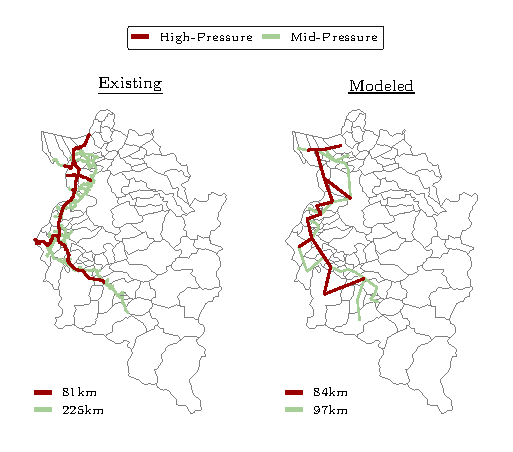
\includegraphics[width=0.8\linewidth]{figures/Comparison.eps}
	\caption{Existing gas networks (high-pressure in red and mid-pressure in green) in Vorarlberg, Austria (left), and its representation in the model (right). Source: \cite{VorarlbergNetz2021}.}
	\label{fig:comparison}
\end{figure}
 
 \subsubsection{Gas demand decline pathways at the community level until 2050}
This section is dedicated to describing the assumptions regarding the development of gas demands at the community level in Vorarlberg, Austria, until 2050. In a first step, we assess total gas demands at the community level in 2018 using information from the open data platform \textit{energiemosaik} \cite{energiemosaik} and our own database (see Section \ref{environment} for data availability). \added[]{Details of the current natural gas demand in Vorarlberg, Austria, is given in} \ref{app_demand}. In a second step, we use the classification of communities regarding the energy demand provided by energiemosaik to estimate the composition of local gas demands. Accordingly, the local gas demand in the community is allocated to one or more of the following sectors of end-use or items: residential, agriculture, industry, SMB, service, and mobility. Building upon this characterization of gas demands by items, the following claim is made: 

\begin{addmargin}[0.75cm]{0pt}
	The composition of the local gas demand at the community level in 2018 determines its development until 2050. Each sector of end-use/item is associated with a decline pathway until 2050. Thus, the total gas demand at the community level until 2050 is described by a linear combination of the individual decline pathways per sector of end-use.
\end{addmargin}
\vspace{0.35cm}

Table \ref{tab:decline_pathway} shows the assumed annual decline rate (and thus decline pathway until 2050) per sector of end-use. We use the naming convention from energiemosaik and use the names Type A, B, C, and D for a combination of different sectors of end-use. We restrict ourselves to four different types (A-D) only. Note that 2050's share in gas demands are rough estimates including higher values if industry and SMBs are located there. For the residential/building heat demand, a linear decrease until 2040 is assumed. 
\begin{table} \centering
	\resizebox{1\textwidth}{!}{
		\renewcommand{\arraystretch}{1.3}
		\begin{tabular}{lccccr}
			\toprule 
			Name & Residential & Industry & SMB & Service &  Decline rate (2050's share)\\\hline
			Type A & \checkmark & & & & Linear until 2040\\
			Type B & \checkmark & \checkmark & \checkmark & & Linear (15\%)\\
			Type C &  &  &  & \checkmark & Linear (20\%)\\
			Type D &  & \checkmark &\checkmark & & Linear (35\%)\\
			\bottomrule
	\end{tabular}}
	\caption{Annual decline rates for different compositions of gas demands at the local community level under the naming convention and sectors of end-use from energiemosaik \cite{energiemosaik}.}
	\label{tab:decline_pathway}
\end{table} 

\subsubsection{Assumptions on the share of green gases in supply and network}

\added{For the modeling it is necessary to estimate the share of green gases up to 2050. In general, this includes the supply of synthetic gas, biomethane and hydrogen. All three are subject to considerable uncertainty. In the Austrian discussion on biomethane and hydrogen, there is a consensus that hydrogen will not be added to natural gas. All national considerations of the gas and hydrogen network infrastructure follow the concept of two separate networks. We take this into account and therefore assume that there are no shares of hydrogen (i.e., no blending of hydrogen) and in the natural gas network. It is therefore not necessary in our specific case to consider the previously mentioned technical limits of hydrogen shares in gas networks. In general, however, such analyses must take into account the technical limits on hydrogen shares. For biomethane, the situation is different compared to hydrogen. It can be assumed that biomethane will be added to natural gas and transported through the gas network. Moreover, it is already added today (see the number of biomethane production facilities in Table \ref{tab:summary_vorarlberg_network}). However, it is uncertain whether large-scale biomethane production in Austria will be profitable in the future. We decide to make a rather conservative estimate of the future production of biomethane within the analyzed network. We assume a threefold increase in production from 2020 to 2030 and a constant remaining production thereafter. We discuss again the role of biomethane within the limitations of the model.}

 \subsection{Data}\label{label:inputs}
 This section shows \deleted{a selection of }the most relevant input data. \added{To replicate the present results, we refer to the code of the model in} \cite{Zwickl_Bernhard_Gas_network_decommissioning_2022} and the dataset at Zenodo \cite{zwicklbernhard_zenodo}. At the same time, we refer to the authors' GitHub repository (details in Section \ref{environment}) for the complete input data. Table \ref{tab:input_costs} shows the cost assumptions for gas networks including the specific investment costs ($c^{inv}_l$) and fixed costs per year ($c^{fix}_l$) for the different gas network levels. Note that 2030 is the assumed year of the decommissiong and refurbishment investment decision for all pipelines within the networks. Additionally, the development of natural gas prices in Europe is taken from the World Energy Outlook 2021 \cite{weoutlook}. The values from the so-called Stated Policies Scenario are taken: \SI{26.28}{EUR \per MWh} in 2030 and \SI{28.33}{EUR \per MWh} in 2050.\footnote{Assuming a linear development between 2030 and 2050.} Revenues are generated in this work on the basis of gas network usage fees. Accordingly, we assume the following values for $p^{loc}_{l,y}$ for each year: \SI{1}{EUR \per MWh} (high-pressure) and \SI{20}{EUR \per MWh} (mid-pressure).\footnote{Note that the currently high natural gas prices are not explicitly considered. However, it can be argued that they are implicitly included as an additional driver for the assumed declining gas demand rates.} 
 
\begin{table}[h]\centering
	\resizebox{1\textwidth}{!}{
	\renewcommand{\arraystretch}{1.3}
	\begin{tabular}{lllrr}
		\toprule 
		Type of costs & Symbol & Network level ($l$) & Value & Source\\\hline
		\multirow{3}{*}{\makecell[l]{Specific investment costs\\(used in Equation \ref{eq:bvalue_ref})}} & \multirow{3}{*}{$c^{inv}_l$} & Transmission & \SI{4600}{EUR\per MW\per km} & \cite{acer}\\
		& & High-pressure & \SI{4000}{EUR\per MW\per km} & \multirow{2}{*}{\cite{EEG}}\\
		& & Mid-pressure & \SI{3000}{EUR\per MW\per km} & \\\hline
		\multirow{3}{*}{\makecell[l]{Fixed costs per year\\(used in Equation \ref{eq:lambda})}} & \multirow{3}{*}{$c^{fix}_l$} & Transmission & \multirow{3}{*}{\SI{2000}{EUR\per MW}} & \multirow{3}{*}{\cite{EEG}}\\ 
		& & High-pressure & & \\
		& & Mid-pressure & & \\
		\bottomrule
	\end{tabular}}
\caption{Cost assumptions of gas networks. The value of specific investment costs of the mid-pressure network level is scaled by the ratio between the existing and the modeled pipeline length (as shown in Figure \ref{fig:comparison}).}
\label{tab:input_costs}
\end{table}

\subsection{Limitation of the model}\label{label:limitation}
Below, we discuss two different limitations of the model, whereas both can be associated with the trade-off decision between (spatial and temporal) granularity and computation time of the model. Besides, nonlinear hydraulic constraints and the book values of compressor stations are not considered.   

\subsubsection{Under-representation of mid-pressure networks and related pipelines}
With an eye on the representation of the mid-pressure gas network presented in Figure \ref{fig:comparison}, it is evident that the corresponding pipelines of the mid-pressure network level are underrepresented in the model. The main reason for this is the (limited) spatial granularity at the community level since large parts of the mid-pressure network are within communities. Within the simplification of the geometry of gas pipelines to the spatial granularity on a community level, mid-pressure gas pipelines within a single community are not considered. This is why the introduction of a tailor-made scaling factor is needed to adjust the specific refurbishment investment costs ($c^{inv}_{mid-pressure}$) accordingly (see Table \ref{tab:input_costs} in Section \ref{label:inputs}). Exemplarily, this scaling factor is $\frac{225}{97}$ (on average) in the case of the mid-pressure network level in Figure \ref{fig:comparison}. 

\subsubsection{Resolution on a monthly basis and associated necessary scaling factors to calculate peak pipeline capacities}
The temporal granularity of the model is limited since it generates results monthly within an individual year. Consequently, again, a scaling factor is needed to link the nodal gas balance constraints (monthly values) with the calculation of needed peak pipeline capacities (Equation \ref{eq:balance}). An hourly resolution could eliminate this calculation process, but, at the same time, one could run into serious computation time matters as the number of equations (i.e., gas balance constraints for node and network level) increases significantly. 

\subsubsection{Assumptions on profitability and volumes of biomethane in the network}
\added[]{Developments in gas demand and biomethane injection are assumed to be exogenous. Both are very difficult to estimate in the context of decarbonizing energy systems. Regarding the assumptions made for natural gas demand, at least the different model runs proposed in this work could increase the significance of the results, as the different model runs can be interpreted as a sensitivity analysis of the gas demand. For the biomethane production and injection into the network, this work assumes conservative volumes as described above. The impact of this assumption on the results is likely to vary between the different model runs proposed here. It depends on how gas demand is treated within the network. In the case of ensured supply (model run 3), therefore, only the network utilization is likely to be overestimated. This is because in this case, a area-wide network remains and biomethane could simply be integrated into the network. Due to the usually shorter distances between biomethane production and demand, this could reduce the network utilization (for example, by comparing the product of transported volumes and distance in} $GWh \cdot km$\added{). In the case without ensure supply (model runs 1 and 2), the biomethane assumption is likely to underestimate the size of the gas network and the volumes transported, as biomethane can be a driver for the use of gas networks. However, in our specific case, this aspect is likely to be small. Two reasons underline this viewpoint. First, as mentioned above, biomethane is usually produced and consumed locally. The transport over long distances is not reasonable mainly due to economic reasons. It would usually require recompression of the biomethane, which, depending on the pressure levels, is energy intensive and therefore very costly. In addition, the model would only underestimate the size of the gas network if biomethane production is higher than gas demand within a node in the network. Essentially, the network only sees the net demand of the node, which is the total demand minus the source. However, it is worth noting that biomethane injection can generally trigger investments in gas networks to enable connection.}

\subsection{Open-source environment and calculation time}\label{environment}
The developed optimization model is implemented in Python 3.8.12 using \deleted[]{the modeling framework} Pyomo version 5.7.3 \cite{hart2017optimization}. It is solved with the solver Gurobi version 9.0.3. For planning the development of gas networks in Vorarlberg, Austria, the model consists of 124155 equations and 98610 continuous variables. It takes on average \SI{3}{\second} to be solved using a computer with an Intel Core i7-8565U with 16 GB of RAM running Microsoft Windows 10 Pro with 64 bit. We use for data analysis the common data format template developed by the Integrated Assessment Modeling Consortium using the open-source Python package pyam \cite{huppmann2021pyam}. Note that all materials used in this study are disclosed as part of the publication on GitHub (\url{https://github.com/sebastianzwickl}). We refer to the repository for the codebase, data collection, and further information.
\section{Results and discussion}\label{results}
This section presents the most relevant results of the analyzed test bed in Vorarlberg, Austria. Section \ref{modelrun1} presents the cost-optimal gas network without an ensured supply of available gas demands (model run 1). Section \ref{modelrun2} puts focus on the (nodal) shadow prices of the cost-optimal gas network without ensured supply (model run 2). Especially, the latter highlights the impact of supplying additional gas demands at the community (or local administrative unit (LAU)) level on the network planning. Section \ref{modelrun3} shows the cost-optimal gas network with ensured supply (model run 3). Section \ref{res:com} compares total costs and shadow prices \replaced[]{with and without}{w/} ensured supply. This includes, the socialization of network costs until 2050. Finally, Section \ref{res:lum} shows the cost-optimal gas network without ensured supply under the lumpiness of gas pipelines. 

\subsection{Cost-optimal gas network without an ensured supply of gas demand (CO)}\label{modelrun1}
In this case, the planning decision is made as follows: if the network operator can treat all energy services equally and thus can decide without restrictions if gas demands are supplied or not, then the gas networks will look like those presented here. Accordingly, it is assumed that competitive alternatives without depedence on gas networks exist for each energy service need. \added[]{Note that the costs of customers not served by the network are not explicitly considered. The shadow prices (discussed in the following section) give a quantitative indication of these costs even without taking them explicitly into account.} Figure \ref{fig:1} shows an overview of the most relevant results in this case. Figure \ref{fig:1} (a) shows the high- and mid-pressure gas networks. Given the existing gas networks (see Figure \ref{fig:comparison}), it is evident that all high-pressure pipelines (in red) are refurbished. At the same time, \SI{59}{\%} of the length of mid-pressure pipelines are refurbished and \SI{41}{\%} are decommissioned. The maximum capacity of the high-pressure network level is \SI{161.92}{} and \SI{40.58}{MW} of the mid-pressure (see Figure \ref{fig:1} (b)). Figure \ref{fig:1} (c) and (d) shows the development of gas demands supplied and not supplied for both pressure/network levels. Particularly, high shares of the mid-pressure demands are covered as a result of comparable high revenues at this pressure level. At the same time, no high-pressure gas demands are covered after 2030. Note that 2030 is the assumed year of the decommissiong and refurbishment investment decision for all pipelines within the networks. 

\begin{figure}[h]
	\centering
	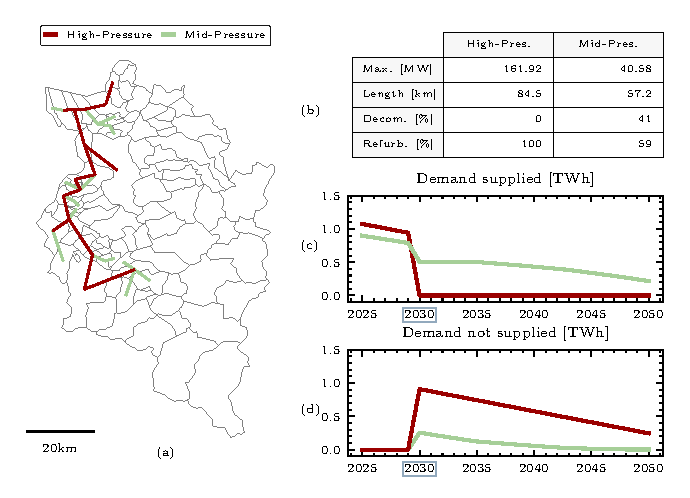
\includegraphics[width=1\linewidth]{figures/modelrun1/overview.eps}
	\caption{Cost-optimal gas networks without ensured supply (model run 1): (a) high- and mid-pressure pipelines, (b) overview of max pipeline capacity, length, and share of decommissioned and refurbished pipeline lengths, (c) demand supplied, and (d) demand not supplied at the high- and mid-pressure network level.}
	\label{fig:1}
\end{figure}

\subsection{Shadow prices for supplying additional gas demands of the cost-optimal gas network without an ensured supply of gas demands}\label{modelrun2}
This section takes the cost-optimal gas network without an ensured supply of gas demands as a starting point and investigates the dual variables and shadow prices of the (nodal) gas balance constraints (see Section \ref{runs}). In this case, emphasis is put on the question: What costs arise and what network adaption is required if the network operator is required to supply an additional gas demand at the nodal level? Since the results of the previous section indicate that mid-pressure gas demands are supplied only (see particularly Figure \ref{fig:1} (c)), this section highlights (nodal) shadow prices of supplying additional gas demands at the mid-pressure network level. \added[]{The shadow prices are the dual variable of the gas demand constraint from Equation \ref{eq:notsupplied}. Here, the shadow price indicates how the value of the objective function would change if additional demand were supplied at a node. Note that these shadow prices refer to network costs only.}\vspace{0.3cm} 



Figure \ref{fig:2} shows shadow prices for LAUs between 2025 and 2050. Figure \ref{fig:2} (a) shows the heatmap of the shadow prices, where the x-axis covers each year between 2025 and 2050 and the y-axis each node potentially connected to the mid-pressure network level. Thereby, each combination (i.e., node and year) is divided on the basis of four categories (i) No expansion (reduced), which means that the network is able to supply the additional gas demand without expansion and thus the objective function value is reduced by the revenues for selling the additional gas demand at the mid-pressure network level; (ii) expansion (reduced), which means that the network needs to be extended to supply the additional gas demand but the objective function value remains reduced but less than by the total revenues for selling gas demand at the mid-pressure network level; (iii) expansion (unaffected), which means that the network must be extended and the objective value is unaffected and remains constant (i.e., shadow price equal to 0), and (iv) expansion (increased), which means that the network needs to be extended and the objective value would be increased (i.e., shadow price greater than 0).

\begin{figure*}[t!]
	\centering
	\begin{subfigure}[t]{0.5\textwidth}
		\centering
		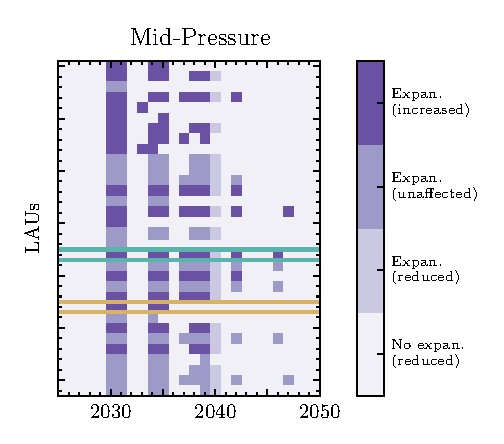
\includegraphics[height=2in]{figures/modelrun2/hm_shdprice.eps}
		\caption{Heat map/capability of the network}
		\label{fig:2a}
	\end{subfigure}%
	~ 
	\begin{subfigure}[t]{0.5\textwidth}
		\centering
		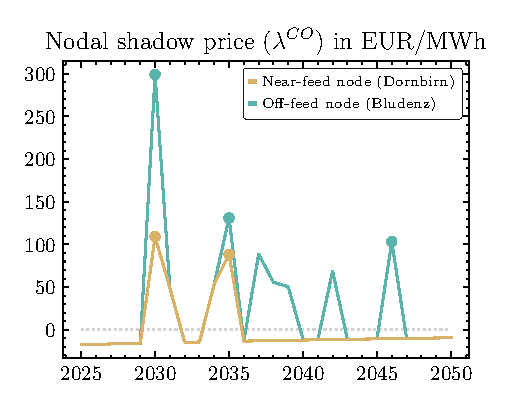
\includegraphics[height=2in]{figures/modelrun2/shadow_example.eps}
		\caption{Near-feed and off-feed node}
	\end{subfigure}
	\caption{Shadow prices for supplying additional gas demands at the mid-pressure network level: (a) heat map identifying the capability of the gas network to supply additional mid-pressure gas demands, and (b) temporal development of the shadow price for a near-feed node (Dornbirn) and a off-feed node (Bludenz).}
	\label{fig:2}
\end{figure*}

 Figure \ref{fig:2} (b) presents the exact numbers of the shadow prices for two representative nodes, namely, a near-feed node (Dornbirn) and an off-feed node (Bludenz). Dornbirn is therefore near the gas supply/source node, and Bludenz is further away from it. The shadow price at the off-feed node has several peaks (three are marked in 2030, 2035, and 2046) and its maximum is \SI{299.2}{EUR\per MWh} in 2030. The near-feed node has two peaks (in 2030 and 2035) and its maximum is \SI{109}{EUR \per MWh} in 2030. Particularly, the development of the near-feed node after 2036 shows the capability of supplying additional gas demands since pipelines capacities are available without expansion.



\subsection{Cost-optimal gas network with an ensured supply of gas demands (ES)}\label{modelrun3}
This section shows the results in the case that the network operator should cover all gas demands within the supply area. Contrary to the previous two sections, no gas demands are not supplied. Figure \ref{fig:result2} shows an overview of the most relevant results in this case. 

\begin{figure}[h]
	\centering
	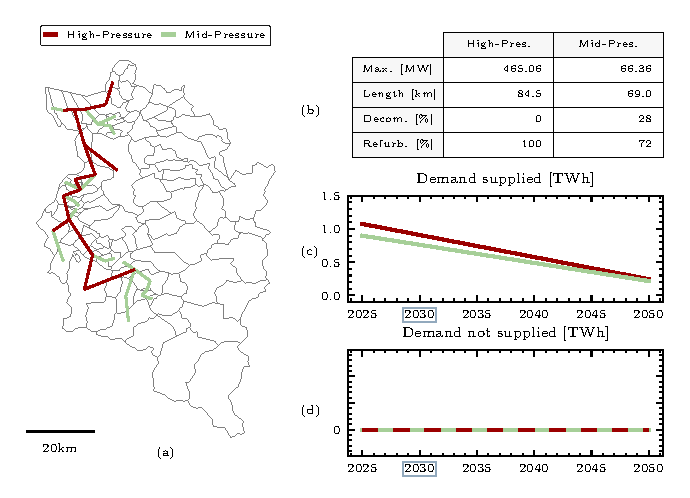
\includegraphics[width=1\linewidth]{figures/modelrun3/network.eps}
	\caption{Cost-optimal gas networks with ensured supply (model run 3): (a) high- and mid-pressure pipelines, (b) overview of max pipeline capacity, length, and share of decommissioned and refurbished pipeline lengths, (c) demand supplied, and (d) demand not supplied at the high- and mid-pressure network level.}
	\label{fig:result2}
\end{figure}

Again, all high-pressure pipelines are refurbished; however, \SI{28}{\%} of mid-pressure pipeline lengths are decommissioned. The maximum capacity of the high-pressure network level is \SI{465.06}{} and \SI{66.36}{MW} of the mid-pressure. Unsurprisingly, the objective function value increases significantly compared with the case without ensured supply. The objective function value increases by \SI{96.29}{MEUR} \added[]{from} \SI{375.1}{MEUR} \added[]{to} \SI{471,39}{MEUR}. This value has great importance and implications for the practical planning of future gas networks. It can serve as a benchmark and is further investigated in the following section, which is dedicated to the comparison of the different cases.

\subsection{Comparison of the cost-optimal gas network with and without ensured supply of gas demands}\label{res:com}
This section compares the cost-optimal gas network with and without an ensured supply of gas demands. We use the following abbreviations, as already used in Table \ref{tabelle:modelruns}: CO for the cost-optimal network without ensured supply and ES with ensured supply. We emphasize the difference in total costs for the network operator and the shadow prices. Figure \ref{fig:result3} shows the most relevant results to compare the two cases, namely, the extra costs in the case of ensured supply (see Figure \ref{fig:result3} (a) and (b)), the distribution of 2030's shadow prices (see Figure \ref{fig:result3} (c)), and shadow price development between 2030 and 2050 for the near-feed and off-feed nodes.

\begin{figure}[h]
	\centering
	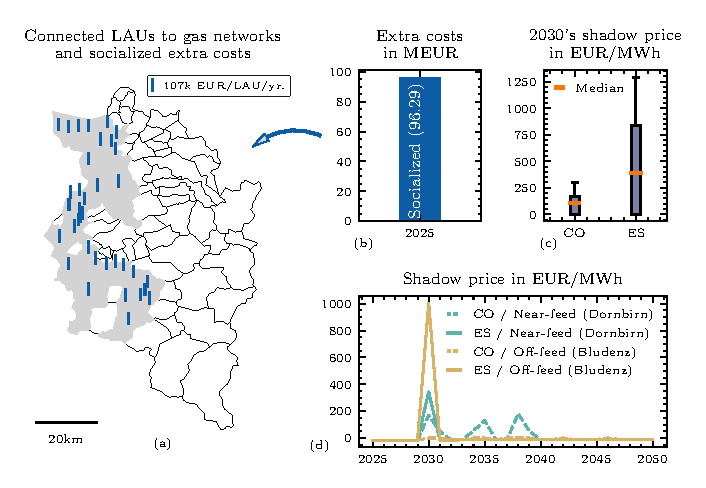
\includegraphics[width=1\linewidth]{figures/Comparison/network.eps}
	\caption{Comparison of the cost-optimal gas network \added[]{with and without} ensured supply of gas demands: (a) and (b) socialized extra costs, (c) 2030's shadow prices, and (d) shadow prices between 2025 and 2050 for the near-feed and off-feed node. CO: Cost-optimal without ensured supply; ES: Cost-optimal with ensured supply.}
	\label{fig:result3}
\end{figure}

As mentioned, the ensured supply of all gas demands within the network results in extra costs of \SI{96.29}{MEUR}. Given an equal allocation to the LAUs and years, this results in extra costs of \SI{107}{kEUR} per LAU and year. This value must be considered as an additional offset to the shadow prices of the cost-optimal network with ensured supply to obtain the effective shadow price and respect the already increasing total costs of the network operator. Nevertheless, even the comparison of 2030's values without this offset shows that the shadow prices in the case with ensured supply increase significantly compared with the case without ensured supply. Particularly, the median raises from approximately \SI{100}{EUR \per MWh} to \SI{400}{EUR \per MWh}. Additionally, the max value raises from approximately \SI{300}{} to \SI{1300}{EUR \per MWh}. This increase in shadow prices is also presented in Figure \ref{fig:result3} (d), where again the near-feed and off-feed nodes are shown. 

\subsection{Cost-optimal gas networks without ensured supply under lumpiness of gas pipelines}\label{res:lum}
This section shows the results of the cost-optimal gas network without ensured supply. Contrary to the results presented above, we consider the lumpiness of gas pipelines in the network operator's planning decision. This analysis completes the results section against the background of two important aspects. First, considering the lumpiness of gas network pipelines increases the significance of the generated results for practical proposals since the network operator's decision is related to choosing specific diameters of gas pipelines. Second, however, the introduction of the lumpiness of gas pipelines extends the previous linear program to a mixed-integer linear program. This is why no dual variables and shadow prices can be obtained. Table \ref{tab:lum} in \ref{app:lum} shows the assumptions for the lumpiness of gas pipelines. We restrict ourselves to 14 different capacities (diameters between 0.1 and \SI{1.3}{\meter}) for both the high- and mid-pressure pressure/network levels. Figure \ref{fig:result4} summarizes the results of the generated gas networks in case of lumpiness. Interestingly, the consideration of lumpiness of gas pipelines leads even in the cost-optimal case network without ensured supply to the decommissioning of \SI{23}{\%} high-pressure and \SI{45}{\%} mid-pressure pipeline length. Furthermore, only gas demands at the mid-pressure network level are supplied (as in Section \ref{modelrun1} and model run 1). Again, all the high-pressure gas demands are not supplied. 

\begin{figure}[h]
	\centering
	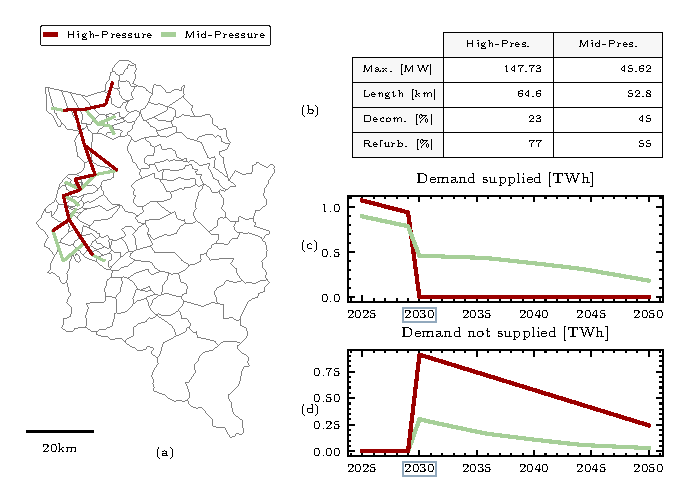
\includegraphics[width=1\linewidth]{figures/lumpiness/network.eps}
	\caption{Cost-optimal gas networks with ensured supply under lumpiness of gas pipelines: (a) high- and mid-pressure pipelines, (b) overview of max pipeline capacity, length, and share of decommissioned and refurbished pipeline lengths, (c) demand supplied, and (d) demand not supplied at the high- and mid-pressure network level.}
	\label{fig:result4}
\end{figure}

Figure \ref{fig:result5} shows a comparison of the results under lumpiness with the previous results of the cost-optimal gas network \replaced[]{with and without}{w/} ensured supply (i.e., CO and ES). Particularly, it shows the impact of lumpiness on an optimal network design decision. In summary, the following interesting findings can be observed:
\begin{itemize}
	\item The cost-optimal network design without ensured supply under lumpiness of gas pipelines increases the total costs (i.e., objective function value) by only 1\% (Figure \ref{fig:result5}, top left) but at the same time the amount of mid-pressure gas demand increases (Figure \ref{fig:result5}, bottom right).
	\item Moreover, the lumpiness of gas pipelines results in both the decommissioning of high shares of the high-pressure network/pressure level (Figure \ref{fig:result5}, top right) and the further decreasing of the maximum pipeline capacity within the network (Figure \ref{fig:result5}, bottom left).
\end{itemize}

\begin{figure}[h]
	\centering
	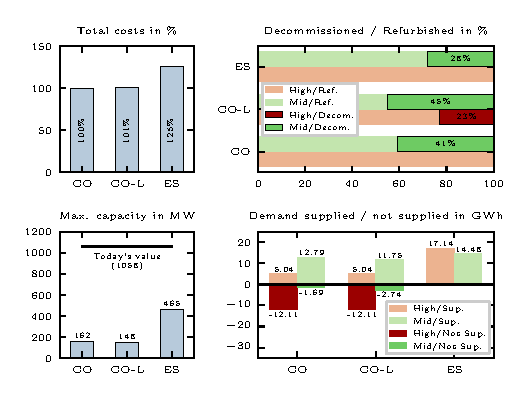
\includegraphics[width=1\linewidth]{figures/synthese/comparison.eps}
	\caption{Results of the cost-optimal gas networks without ensured supply under lumpiness of gas pipelines (CO-L). Top left: Comparison of the total costs. Top right: Decommissioning and refurbishment decision at the mid- and high-pressure network level. Bottom left: Maximum pipeline capacity. Bottom right: Mid- and high-pressure gas demand that is supplied or not.}
	\label{fig:result5}
\end{figure}

\section{Conclusions and policy implications}\label{conclusions}
The ongoing defossilization of the provision of energy services leads to declining natural gas demands. That and the expectation of very limited economically useable potentials of green gases, a transparent and critical discussion regarding the future development of existing gas networks without any taboos is needed. This work investigates the trajectory of gas networks in a test bed until 2050, including the decision of decommissioning parts of the existing gas networks. Particularly, the analysis is conducted out from the network operator's perspective and shows different network decommissioning or refurbishment options under the decision of supplying or not supplying available gas demands.\vspace{0.3cm}

We find that smaller gas networks (in terms of pipeline capacity and network length) are needed in the future regardless of ensured supply. However, the results indicate a wide range of possible network developments until 2050 resulting from the handling of gas demand. This reveals crucial trade-off decisions for gas network operators in the future and includes, the decommissioning decision of gas pipelines despite possible gas demand. Moreover, the conducted analysis of shadow prices of the local gas balance constraint shows that a balance/trade-off between the cost-optimal gas network design with and without ensured supply could lead to a robust and economically competitive future of gas networks.\added[]{Ultimately, however, the size of the gas networks is determined not only by the demand side but also by the feed-in side and, thus, in the future, by the quantities in which green gases are economically available.}\vspace{0.3cm}

Nevertheless, the results demonstrate that it is necessary to socialize network operators' costs under the remaining consumers connected to the network in the future. This fact has several important implications. First and foremost, that brings an additional cost component to consumers \added{(particularly relevant for the hard-to-abate energy sectors)}, which needs to be considered when dealing with the profitability of sustainable alternatives substituting natural gas. Analyses elaborating on trade-offs between natural gas and other sustainable supply options are often neglecting this network-related cost component, which brings a bias into the decision process.\vspace{0.3cm}

\added{However, this research has several limitations and further improvements could be done regarding different aspects. In particular, f}uture work should investigate the development of gas demand in different sectors (e.g., building heat and industry) in more detail, bringing further insights into gas networks requirements and topologies until 2050. Additionally, the role of green gases could be enhanced. In particular, further work should include different types of gas pipelines associated not only with the network/pressure level but also with the quality of the gas transported.

\section*{Declaration of interests}
None.
\section*{Declaration of Competing Interest}
The authors report no declarations of interest.
\section*{Acknowledgments}
This project has received funding from the European Union's Horizon 2020 Research and Innovation Programme under Grant Agreement No. 835896. The authors acknowledge TU Wien Bibliothek for financial support through its Open Access Funding Programme.

\bibliography{mybibfile}
\appendix
\setcounter{table}{0}
\setcounter{figure}{0}

\section{Overview of the model equation}\label{app_overview}

\begin{sidewaystable}
	\centering
	\setlength{\extrarowheight}{.5em}
	\resizebox{1\textwidth}{!}{
		\begin{tabular}{cclll}
			\toprule
			\multicolumn{2}{c}{Equation} & \multicolumn{3}{c}{Qualitative/high-level explanation of the mathematical formulation}\\\cmidrule(lr){1-2}\cmidrule(lr){3-5}
			Number & Dimension & Type & Keyword & Description\\\hline
			\ref{objective} & 1 & Economic & Objective &  Minimize gas network operator's total costs\\
			\ref{eq:capex} & 1 & Economic  & Capex &  Capital cost of the gas pipelines\\
			\ref{eq:opex} & 1 & Economic & Opex & Fixed operating costs of gas pipelines\\
			\ref{eq:total_book_value} & ($p \times l \times y$) & Economic & Book values & Book value per gas pipeline, network level and year\\
			\ref{eq:revenues} & ($n \times l \times y \times m$) & Economic & Revenues & Revenues for supplying gas demand through network charge\\
			\ref{bound1}, \ref{bound2} & ($p \times l \times y$) & Technical & Gas transport & Restriction of the gas transport per gas pipeline, network level and year\\
			\ref{eq:balance} & ($n \times l \times y \times m$) & Technical & Gas balance & Gas balance constraint per node, network level, year and month\\
			\ref{eq:demand} &  ($n \times l \times y \times m$) & Technical & Gas demand & Total gas demand as sum of local demand and delivered gas\\
 			\ref{eq:source} &  ($n \times l \times y \times m$) & Technical & Gas source & Total gas source as sum of local production and gas delivered\\
			\bottomrule
	\end{tabular}}
	\caption{\added{Overview of the model's mathematical formulation. Abbreviations: Gas pipeline (p), Network level (l), Node (n), Year (y), Month (m)}}
	\label{tab:brief}
\end{sidewaystable}

\section{Current natural gas demands in Vorarlberg, Austria}\label{app_demand}
Figure \ref{fig:comp} shows current natural gas demands in Vorarlberg, Austria. The left subfigure shows natural gas demands in Vorarlberg, Austria, in 2018 and 2025. Open data and information from the internal database \cite{EEG} are used to split 2018's values into industry and (building) heating. The values are available at the provincial level (i.e., Vorarlberg, Austria). The 2025's values are calculated bottom-up. That means that we use data on natural gas demands at the community level (between 2018 and 2025). Note that the difference between 2018's and 2025's gas demands reflects the lack of gas demand data at the community level only. 

\begin{figure}[h]
	\centering
	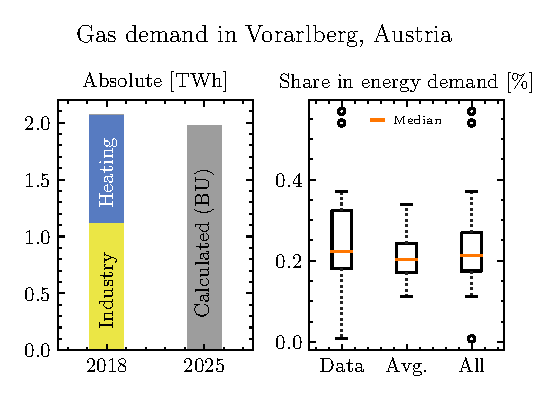
\includegraphics[width=0.75\linewidth]{figures/Comparison_of_the_demand.eps}
	\caption{Overview of gas demands in 2018 and 2025 (left) and share of natural gas in total energy demand (right). Data: open data available; Avg.: shares calculated based on the average gas demand per capita in Vorarlberg, Austria; All: Data and Avg. combined.}
	\label{fig:comp}
\end{figure}

The right subfigure indicates the approach to calculating gas demands if no open data are available. It shows the share of natural gas demands in energy demand at the community level. The first item (Data) shows the distribution for those communities where data are available. The second item (Avg.) shows the distribution of gas demand shares using the average value of gas demand per capita in Vorarlberg, Austria. This calculation process based on the average gas demand is used for communities where no data are available. The third item (All) shows the distribution of gas demand shares for all communities.



\section{Assumptions regarding lumpiness of gas pipelines}\label{app:lum}
Similar to \cite{von2006reform}, we assume a simplified relationship between the diameter of gas pipelines and their capacities. Accordingly, we assume that the capacity of high- and mid-pressure gas pipelines increases by 2.5 times the power of the diameter. Table \ref{tab:lum} summarizes the set of potential diameters and the corresponding calculated capacity. 

\definecolor{Gray}{gray}{0.95}
\begin{table}[h]
	\centering
	\scalebox{1}{
			\renewcommand{\arraystretch}{1.4}
			\begin{tabular}{c|c}
					Diameter in meters & Pipeline capacity in MW\\\hline
					0.1 & 0.82\\
					0.2 & 4.62\\
					0.3 & 12.72\\
					0.4 & 26.11\\
					0.5 & 45.62\\
					0.6 & 71.96\\
					0.7 & 105.8\\
					0.8 & 147.73\\
					0.9 & 198.31\\
					1.0 & 258.07\\
					1.1 & 327.51\\
					1.15 & 366.0\\
					1.2 & 407.09\\
					1.3 & 497.27\\
			\end{tabular}}
	\caption{Set of diameters of gas pipelines and assumed pipeline capacity.}
	\label{tab:lum}
\end{table}
\end{document}